% !TeX root = ../../Book1.tex
% 纲要标题：### 5.5 群作用、单值与覆盖的重建
% 纲要位置：几何学计划纲要.md，第 306 行。
% 正文状态：初稿；尚未正式审核。

% 纲要内容开始
% 
% * 适当不连续作用构造商覆盖
% * 纤维上的置换单值
% * 由单值数据重建覆盖
% * 环面、曲面及图覆盖的计算
% 
% ---
% 
% 纲要内容结束

\section{群作用、单值与覆盖的重建}
\label{g1:sec:0505}

沿底空间的道路行走时，覆盖中的起点一旦选定，整条提升就被确定了。如果底空间中的道路回到原点，提升却可能到达同一纤维的另一个点。于是环路给出纤维的一次置换。上一节用子群描述一个连通覆盖；本节把纤维的所有点一起保留，用这种置换记录整个覆盖，也允许覆盖不连通。

\subsection{适当不连续作用构造商覆盖}
\label{g1:subsec:0505:01}

第四章已经提醒，群轨道的商不一定是良好的几何空间：有理平移的商甚至只有平凡拓扑。要得到覆盖，所需条件相当具体：每一点应有一个小邻域，它的不同平移副本互不相交。这样，一个小邻域在取商时只被复制和识别，不会在内部折叠。

\begin{definition}[用于覆盖的适当不连续作用]\label{g1:def:properly-discontinuous-covering}
	设群 \(\Gamma\) 通过同胚左作用于拓扑空间 \(E\)。本节称该作用\term[shidangbulianxuzuoyong]{适当不连续}[properly discontinuous]，如果对每个 \(e\in E\)，都存在开邻域 \(V\ni e\)，使
	\[
		gV\cap V=\varnothing\qquad(g\in\Gamma,\ g\ne1).
	\]
	此约定包含自由性：若 \(ge=e\)，上述邻域立即迫使 \(g=1\)。有的文献允许非平凡点稳定子群而使用同一术语，应用其结论时需要核对定义。
\end{definition}

\begin{proposition}[作用的商是覆盖]\label{g1:prop:action-quotient-cover}
	设 \(\Gamma\) 在非空拓扑空间 \(E\) 上有上述作用，商集 \(E/\Gamma\) 取商拓扑。则轨道映射 \(q:E\rightarrow E/\Gamma\) 为覆盖。若 \(E\) 连通，则这个覆盖的甲板变换群恰为给定的 \(\Gamma\)；若 \(E\) 还单连通，则它是一个万有覆盖。
\end{proposition}
\begin{proof}
	对任意开集 \(O\subseteq E\)，有
	\[
		q^{-1}(q(O))=\bigcup_{g\in\Gamma}gO,
	\]
	右边开，故 \(q\) 为开映射。取定义中的 \(V\)。它的各个平移 \(gV\) 两两不交：若 \(gV\cap hV\ne\varnothing\)，则 \(h^{-1}gV\cap V\ne\varnothing\)，从而 \(g=h\)。由于 \(q|_V\) 连续、单射、开，且映满 \(q(V)\)，它为同胚；每个 \(q|_{gV}\) 同样为同胚。因此
	\[
		q^{-1}(q(V))=\bigsqcup_{g\in\Gamma}gV
	\]
	正是覆盖的局部形式。

	每个 \(g\) 保持轨道，故为甲板变换。反过来，若 \(E\) 连通且 \(T\) 是任意甲板变换，固定 \(e\in E\)，由同纤维就是同轨道，可找唯一 \(g\) 使 \(T(e)=ge\)。映射 \(T\) 与 \(g\) 都是 \(q\) 到自身的提升，由\cref{g1:prop:deck-determined}，在一点相等便处处相等。所以没有额外的甲板变换。单连通时，按万有覆盖的定义即得最后结论。
\end{proof}

整数群在 \(\mathbb R\) 上的平移满足此条件，因为长度小于 \(1\) 的开区间与其非零整数平移不交。由 \(t\mapsto e^{2\pi it}\) 可识别 \(\mathbb R/\mathbb Z\cong S^1\)，得到圆周的万有覆盖。反之，\(\mathbb Q\) 的平移在任何开区间中都有非零的小平移与自身相交，恰好失去这一条件。反射 \(x\mapsto-x\) 的作用在原点有稳定子群，其商映射 \(\mathbb R\rightarrow[0,\infty)\) 在原点附近也不是覆盖：任一含原点的开区间都包含两个被识别的点，不能成为一张同胚覆盖片。

\begin{proposition}[万有覆盖上的基本群作用]\label{g1:prop:universal-deck-discontinuous}
	设 \(X\) 非空、道路连通、局部道路连通且半局部单连通，\(\widetilde X\) 是从基点 \(x_0\) 出发的道路类万有覆盖，\(G=\pi_1(X,x_0)\)。由
	\[
		L_g[\alpha]=[\gamma*\alpha]\qquad(g=[\gamma])
	\]
	给出的 \(G\) 左作用适当不连续，而且在每个纤维上自由且传递。
\end{proposition}
\begin{proof}
	这些映射及其群乘法由\cref{g1:thm:normal-covering-deck}给出。若道路 \(\alpha,\beta\) 终点相同，取 \(g=[\beta*\bar\alpha]\)，便有 \(L_g[\alpha]=[\beta]\)，故作用在纤维上传递；自由性来自甲板变换由一点决定。

	取底空间一个连通的均匀覆盖邻域 \(U\)，并取上方一张片 \(V\)。每个 \(L_g\) 把 \(V\) 映到 \(U\) 上方的一张片，因为它保持投影，且片可由道路提升从其中一点得到。若 \(L_gV\) 与 \(V\) 相交，两片必相同。此时投影在 \(V\) 上单射，迫使 \(L_g|_V=\operatorname{id}_V\)，再由甲板变换的确定性得到 \(g=1\)。因此 \(V\) 的不同群平移两两不交。
\end{proof}

这里的“均匀覆盖邻域”指其原像分解成同胚覆盖片的开邻域；连通的选择由底空间局部道路连通保证。它与前一节道路类构造中的好邻域是同一类局部工具。

\subsection{纤维上的置换单值}
\label{g1:subsec:0505:02}

现在固定任意覆盖 \(p:E\rightarrow X\) 和基点 \(x_0\in X\)，令 \(S=p^{-1}(x_0)\)。这一纤维是离散空间，但其点不需要预先排列成编号。我们把“从哪一点出发，沿环路以后到哪一点”作为置换的定义。

\begin{proposition}[单值的右作用]\label{g1:prop:monodromy-action}
	设 \(p:E\rightarrow X\) 为覆盖，\(x_0\in X\)，\(G=\pi_1(X,x_0)\)。对 \(s\in S=p^{-1}(x_0)\) 与 \(g=[\gamma]\in G\)，定义
	\[
		s\cdot g=\widetilde\gamma_s(1),
	\]
	其中 \(\widetilde\gamma_s\) 是从 \(s\) 出发的唯一道路提升。则此公式良定义，并构成 \(G\) 在 \(S\) 上的右作用。这称为覆盖的\term[danzhizuoyong]{单值作用}[monodromy action]。
\end{proposition}
\begin{proof}
	\cref{g1:cor:lifted-path-homotopy}保证同伦的环路从同一纤维点提升后有相同终点，所以结果只依赖 \(g\)。常值道路的提升常值，故 \(s\cdot1=s\)。先走 \(\gamma\) 再走 \(\eta\) 时，可以先提升 \(\gamma\)，再从其终点提升 \(\eta\)；两段拼接是 \(\gamma*\eta\) 的提升，由唯一性就是全部提升。因此
	\[
		(s\cdot g)\cdot h=s\cdot(gh).
	\]
	沿反路提升把终点送回起点，所以每个 \(g\) 给出的映射均为置换，逆置换由 \(g^{-1}\) 给出。
\end{proof}

本书先走左边道路的乘法约定，自然产生右作用。若把 \(s\mapsto s\cdot g\) 记作置换 \(M_g\)，并按通常函数复合记乘法，则 \(M_{gh}=M_h\circ M_g\)。若希望得到按通常复合的群同态 \(G\rightarrow\operatorname{Sym}(S)\)，应取 \(g\mapsto M_{g^{-1}}\)。后面直接使用右作用等式，避免在两个约定之间来回转换。

\begin{proposition}[轨道、稳定子群与覆盖的连通性]\label{g1:prop:monodromy-components}
	设 \(X\) 非空、道路连通且局部道路连通，\(p:E\rightarrow X\) 为覆盖，\(S=p^{-1}(x_0)\)。
	\begin{enumerate}
		\item \(S\) 的单值轨道与 \(E\) 的连通分支一一对应。因此 \(E\) 连通当且仅当单值作用传递。
		\item 对 \(s\in S\)，其稳定子群是 \(p_*\pi_1(E,s)\subseteq G\)。
		\item 设该子群为 \(H\)。轨道 \(sG\) 与陪集集合 \(H\backslash G=\{Hg:g\in G\}\) 右等变双射，对应为 \(Hg\mapsto s\cdot g\)。
	\end{enumerate}
\end{proposition}
\begin{proof}
	由覆盖的局部形式，\(E\) 局部道路连通，故由\cref{g1:thm:locally-path-components}，连通分支就是道路分支。每个分支都遇到 \(S\)：从任一点的投影沿道路到 \(x_0\)，提升后就在同一分支中到达 \(S\)。两点 \(s,t\in S\) 能在 \(E\) 中用道路相连，当且仅当某个底空间环路的提升从 \(s\) 到 \(t\)，这正是二者属于同一单值轨道，得到第一项。

	等式 \(s\cdot g=s\) 意味着对应提升是闭路；由\cref{g1:cor:closed-lift-criterion}，这恰好等价于 \(g\in p_*\pi_1(E,s)\)，得到第二项。最后，
	\[
		s\cdot g=s\cdot h
		\quad\Longleftrightarrow\quad gh^{-1}\in H
		\quad\Longleftrightarrow\quad Hg=Hh.
	\]
	故陪集对应良定义且单射，满射由轨道的定义得到；右乘的相容性也直接来自作用等式。
\end{proof}

例如 \(z\mapsto z^n\)（\(n\ge1\)）的纤维可标为 \(s_j=e^{2\pi ij/n}\)，\(j\in\mathbb Z/n\mathbb Z\)。一周正向环路从 \(s_j\) 提升为 \(e^{2\pi i(t+j)/n}\)，终点是 \(s_{j+1}\)。所以基本群的生成元在纤维上作一个 \(n\)-循环，其稳定子群为 \(n\mathbb Z\)。一个局部选出的 \(n\) 次根沿圆周继续一周以后会改变分支，这就是单值作用所记录的现象。

\subsection{由单值数据重建覆盖}
\label{g1:subsec:0505:03}

反过来，若只给一个集合 \(S\)，以及底空间环路如何置换 \(S\) 的规则，能否找回覆盖？万有覆盖已经把每条道路的行走历史保存为道路类；把历史改变时纤维编号应如何改变一并规定，就能作出所需商空间。

\begin{theorem}[由右群作用重建覆盖]\label{g1:thm:monodromy-reconstruction}
	设 \(X\) 非空、道路连通、局部道路连通且半局部单连通，固定 \(x_0\)，令 \(G=\pi_1(X,x_0)\)，\(\widetilde p:\widetilde X\rightarrow X\) 为道路类万有覆盖。对任意非空右 \(G\) 集合 \(S\)，赋予 \(S\) 离散拓扑，并在 \(S\times\widetilde X\) 上定义左作用
	\[
		g\cdot(s,u)=(s\cdot g^{-1},L_g u).
	\]
	则轨道商
	\[
		E_S=(S\times\widetilde X)/G,\qquad p_S([s,u])=\widetilde p(u)
	\]
	是 \(X\) 上的覆盖。其基点纤维自然等于 \(S\)，单值作用就是原给定右作用。每个非空覆盖均由此得到，两个这样的覆盖同构当且仅当其纤维右 \(G\) 集合同构。
\end{theorem}
\begin{proof}
	先核验群作用方向。连续施以 \(h\) 再施以 \(g\)，第一坐标变为 \(s\cdot h^{-1}g^{-1}=s\cdot(gh)^{-1}\)，第二坐标变为 \(L_{gh}u\)，所以确为左作用。每个作用映射为同胚，且保持 \(\widetilde p(u)\)，因此 \(p_S\) 良定义且连续。商映射 \(q:S\times\widetilde X\rightarrow E_S\) 开，证明与\cref{g1:prop:action-quotient-cover}相同。

	取连通的均匀覆盖邻域 \(U\subseteq X\) 和万有覆盖的一张片 \(V\)。由\cref{g1:prop:universal-deck-discontinuous}，其他各片恰为 \(L_gV\)，而且指标 \(g\) 唯一。对每个 \(s\in S\)，令 \(W_s=q(\{s\}\times V)\)。这些集合开，并且 \(q\) 将 \(\{s\}\times V\) 同胚地映到 \(W_s\)：若其中两点被识别，则某个 \(L_gV\) 与 \(V\) 相交，迫使 \(g=1\)。同样的论证说明不同 \(s\) 给出的 \(W_s\) 不交。若 \(u=L_gv\)、\(v\in V\)，轨道关系给出
	\begin{equation}\label{g1:eq:associated-cover-relation}
		[s,L_gv]=[s\cdot g,v],
	\end{equation}
	所以这些 \(W_s\) 覆盖 \(p_S^{-1}(U)\)，且每个 \(p_S|_{W_s}\) 与 \(\widetilde p|_V\) 对应，为到 \(U\) 的同胚。这证明覆盖性质。

	记万有覆盖基点为 \(\widetilde x_0=[e_{x_0}]\)。纤维点写成 \([s,\widetilde x_0]\) 的方式唯一，故基点纤维与 \(S\) 相同。从此点提升代表 \(g\) 的环路 \(\gamma\)，可以使用道路 \(t\mapsto[s,\widetilde\gamma(t)]\)，其中 \(\widetilde\gamma\) 从 \(\widetilde x_0\) 出发。其终点为
	\[
		[s,L_g\widetilde x_0]=[s\cdot g,\widetilde x_0],
	\]
	所以单值恰为指定的右作用。

	再设 \(p:E\rightarrow X\) 是任意覆盖，\(S=p^{-1}(x_0)\) 取其单值作用。对每个 \(s\)，由\cref{g1:thm:lifting-criterion}，\(\widetilde p\) 有唯一连续提升 \(F_s:\widetilde X\rightarrow E\) 满足 \(F_s(\widetilde x_0)=s\)：定义域道路连通、局部道路连通且单连通，因此基本群包含条件自动成立。具体地，\(F_s([\alpha])\) 是 \(\alpha\) 从 \(s\) 出发的提升终点。映射 \(F(s,u)=F_s(u)\) 在离散积上连续。先从 \(s\cdot g^{-1}\) 提升 \(\gamma\)，会回到 \(s\)，然后提升 \(\alpha\)，故
	\[
		F(s\cdot g^{-1},L_g[\alpha])=F(s,[\alpha]).
	\]
	它因而下降为连续映射 \(\bar F:E_S\rightarrow E\)，并保持到底空间的投影。

	给定 \(x\in X\) 及一条从 \(x_0\) 到 \(x\) 的道路 \(\alpha\)，沿 \(\alpha\) 提升给出纤维 \(S\rightarrow p^{-1}(x)\) 的双射，其逆由反路提升给出。另一方面，\(E_S\) 中 \(x\) 上方的点也唯一写成 \([s,[\alpha]]\)。所以 \(\bar F\) 在每个纤维上双射，因而全局双射。它在足够小的共同均匀覆盖邻域上逐片等于两张同胚片之间的坐标对应，故为局部同胚；双射局部同胚是同胚。因此找回了原覆盖。

	最后，覆盖同构限制到基点纤维后与道路提升相容，故是右 \(G\) 集合的同构。反过来，右等变双射 \(\phi:S\rightarrow S'\) 使 \((s,u)\mapsto(\phi(s),u)\) 与轨道关系相容，下降为 \(E_S\rightarrow E_{S'}\) 的同构，逆映射由 \(\phi^{-1}\) 给出。
\end{proof}

若允许空总空间，空集合也对应一个空的局部覆盖；本章覆盖按满射定义，所以定理明确使用非空 \(S\)。在连通情形，传递右 \(G\) 集合写成 \(H\backslash G\)，便恢复上一节的子群分类。这里的重建还保留了不同轨道，因此同时处理不连通覆盖。

\begin{corollary}[甲板变换与等变置换]\label{g1:cor:deck-centralizer}
	在上一定理的假设下，任一覆盖 \(E\rightarrow X\) 的甲板变换群，等于其纤维 \(S\) 上与全部单值置换交换的置换群。
\end{corollary}
\begin{proof}
	甲板变换将从 \(s\) 出发的道路提升送到从 \(T(s)\) 出发的提升，因此 \(T(s\cdot g)=T(s)\cdot g\)。反过来，每个满足此等式的纤维置换由定理的重建公式扩张为甲板变换。扩张唯一：每一点都是某条从基点纤维出发的提升道路的终点，而该终点的像已由纤维置换决定。限制与扩张保持函数复合，所以给出群同构。
\end{proof}

单值作用和甲板变换作用因此不是同一件事。前者由底空间环路推动纤维点，后者是整个覆盖保持投影的对称；后者必须与前者交换。

\subsection{环面、曲面及图覆盖的计算}
\label{g1:subsec:0505:04}

先看环面。由\cref{g1:prop:product-fundamental}，\(\pi_1(T^2)\cong\mathbb Z^2\)，而逐坐标指数映射
\[
	P:\mathbb R^2\longrightarrow T^2,\qquad P(u,v)=(e^{2\pi iu},e^{2\pi iv})
\]
为万有覆盖：两个圆周覆盖片的积给出覆盖局部形式，\(\mathbb R^2\) 凸而单连通。甲板群是整数平移。对子群 \(H\le\mathbb Z^2\)，得到连通覆盖 \(\mathbb R^2/H\rightarrow T^2\)，纤维为 \(H\backslash\mathbb Z^2\)。因为底群交换，这些连通覆盖全部正规。

\begin{example}[一个六叶环面覆盖]\label{g1:exm:torus-six-cover}
	取 \(H=\langle(2,0),(1,3)\rangle\)。线性映射 \(A(u,v)=(2u+v,3v)\) 将 \(\mathbb Z^2\) 映到 \(H\)，并诱导同胚 \(\mathbb R^2/\mathbb Z^2\rightarrow\mathbb R^2/H\)。所以相应覆盖可写成
	\[
		f:T^2\longrightarrow T^2,\qquad f(z,w)=(z^2w,w^3).
	\]
	每个陪集都有唯一代表 \((r,s)\)，其中 \(r=0,1\)，\(s=0,1,2\)：先用 \((1,3)\) 把第二坐标约化到这三个值，再用 \((2,0)\) 约化第一坐标；若两个代表之差在 \(H\)，第二坐标差迫使 \((1,3)\) 的系数为零，再由第一坐标得到两代表相同。因此叶数为 \(6\)。

	令 \(e_1=(1,0),e_2=(0,1)\)。商群中 \(2e_1=0\)、\(e_1+3e_2=0\)，所以 \(e_1=-3e_2\)，全群由 \(e_2\) 生成且有六个元素，即甲板群为 \(\mathbb Z/6\mathbb Z\)。沿两个圆周生成环路的单值分别是陪集加 \(e_1,e_2\)，在这一循环编号下分别为加 \(3\)、加 \(1\)。这同时给出了覆盖公式、叶数、单值与甲板群。
\end{example}

对由标准边字
\[
	[a_1,b_1]\cdots[a_g,b_g],\qquad [a,b]=aba^{-1}b^{-1},
\]
得到的可定向多边形曲面模型 \(\Sigma_g\)，先对其 \(2g\) 条边组成的一点并图使用\cref{g1:prop:graph-fundamental}，再由\cref{g1:prop:attach-disk}沿该边字附着圆盘，就得到以这些生成元和该关系为展示的基本群（\(g\ge1\)）。构造 \(n\) 叶覆盖时，可在 \(S=\{1,\ldots,n\}\) 上指定各生成元的右置换；唯一需要检查的关系是按该边字依次作用后恒等。这保证自由群作用通过所展示的商群下降，再由\cref{g1:thm:monodromy-reconstruction}得到覆盖。生成置换的轨道决定覆盖的连通分支。这里使用的是明确的多边形模型及其关系，不需要预先知道所有紧曲面的分类。

例如 \(g\ge1\) 时，令 \(a_1\) 作 \(n\)-循环，其余 \(a_i,b_i\) 全部恒等。每个交换子作用都恒等，所以关系满足；\(n\)-循环使作用传递，故得到连通 \(n\) 叶覆盖。单值通过满同态 \(\pi_1(\Sigma_g)\rightarrow\mathbb Z/n\mathbb Z\) 的正则作用给出，稳定子群就是该同态的核，因而此覆盖正规，甲板群为 \(\mathbb Z/n\mathbb Z\)。

\begin{example}[图覆盖中单值与甲板群的差别]\label{g1:exm:three-sheet-graph}
	设 \(B\) 为两个圆周 \(a,b\) 在一点相接的图，\(\pi_1(B)=F(a,b)\)。在三个纤维点上规定右置换
	\[
		s\cdot a=(12)(s),\qquad s\cdot b=(23)(s).
	\]
	自由群没有关系，故这给出一个右作用：一个字从左到右逐个作用即可。构造覆盖图时，在顶点 \(1,2,3\) 之间，为每个 \(s\) 放一条从 \(s\) 到 \(s\cdot a\) 的有向 \(a\)-边，再放一条从 \(s\) 到 \(s\cdot b\) 的有向 \(b\)-边。每条边按参数同胚地映到基图相应边的内部。

	在每个顶点附近，各有一条 \(a\)-边进入、一条 \(a\)-边离开，以及对应的两条 \(b\)-半边；环边也分别贡献进入、离开的半边。因此顶点的小星形邻域同胚地映到基图基点的小星形邻域，边内部也显然满足覆盖条件，得到三叶图覆盖。两次换位生成传递作用，所以覆盖连通。图有三个顶点和六条边，由\cref{g1:prop:graph-fundamental}，其基本群为秩 \(6-3+1=4\) 的自由群。

	单值置换生成 \(S_3\)，但甲板群平凡。事实上，若置换 \(T\) 同时与 \((12)\)、\((23)\) 交换，它必须分别保留二者唯一的不动点 \(3,1\)，于是也固定 \(2\)，所以 \(T=\operatorname{id}\)。由\cref{g1:cor:deck-centralizer}，覆盖没有非平凡甲板变换。覆盖连通只说明单值传递，并不保证甲板变换能把任意纤维点送到另一个。
\end{example}

\begin{figure}[htbp]
	\centering
	% !TeX root = ../Book1.tex
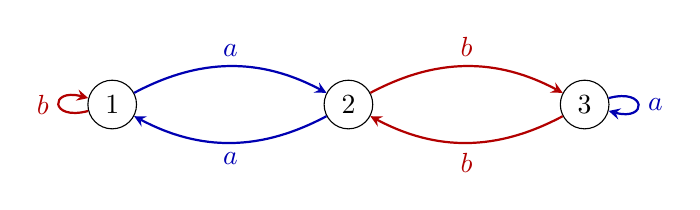
\begin{tikzpicture}[x=1cm,y=1cm,>=stealth]
	\node[circle,draw,minimum size=6mm] (v1) at (0,0) {\(1\)};
	\node[circle,draw,minimum size=6mm] (v2) at (3,0) {\(2\)};
	\node[circle,draw,minimum size=6mm] (v3) at (6,0) {\(3\)};
	\draw[blue!70!black,thick,->] (v1) to[bend left=28] node[above] {\(a\)} (v2);
	\draw[blue!70!black,thick,->] (v2) to[bend left=28] node[below] {\(a\)} (v1);
	\draw[red!70!black,thick,->] (v2) to[bend left=28] node[above] {\(b\)} (v3);
	\draw[red!70!black,thick,->] (v3) to[bend left=28] node[below] {\(b\)} (v2);
	\draw[red!70!black,thick,->] (v1) to[loop left] node[left] {\(b\)} (v1);
	\draw[blue!70!black,thick,->] (v3) to[loop right] node[right] {\(a\)} (v3);
\end{tikzpicture}

	\caption{二圈图的三叶覆盖。蓝色边标记 \(a\)，红色边标记 \(b\)；同一对顶点间的两条反向边是两条不同的边。每个顶点都有各标记的一入一出，纤维置换分别为 \((12)\) 与 \((23)\)。}
	\label{g1:fig:three-sheet-graph}
\end{figure}

这些例子显示两种计算可以相互检查。先从图形或粘合求基本群，再用它在纤维上的作用建立覆盖；反过来，提升终点、叶数和甲板变换又能检验原来的群与关系。关于覆盖、群作用和图的进一步阅读，可参阅\cite[Section 1.3; Section 1.A]{Hatcher2002}。
